正如我们刚才看到的,对共享数据的并发(同时)访问是一个性能杀手。直观地说,这是有意义的:为了避免数据竞争,在给定的时间内只有一个线程可以操作共享数据。我们可以使用互斥量来完成这个任务,如果有原子操作的话,也可以使用原子操作。无论哪种方式,当一个线程递增共享变量时,其他所有线程都必须等待。我们在上一部分的测试结果也证实了这一点。

然而,在根据观察和实验采取任何行动之前,要准确地理解我们测量了什么,以及可以确定地得出什么结论。

很容易描述所观察到的情况:多个线程同时递增一个共享变量根本没有扩展性,甚至比只使用一个线程还要慢,原子共享变量和互斥保护的非原子变量都是如此。我们没有尝试测试对非原子变量的无保护访问,因为这样的操作会导致未定义行为和不正确的结果。我们还知道,对特定于线程(非共享)变量的无保护访问,可以很好地随着线程的数量而扩展,至少直到我们饱和了内存带宽(这只会发生在我们写大量数据的时候;对于单个变量来说,这不是问题)。批判性地、不带偏见地分析实验结果是一项非常重要的技能,再次说明:有保护的访问共享数据很慢,而无保护的访问非共享数据很快。如果由此得出共享数据会使程序变慢的结论,就需要做出一个假设:\textbf{共享数据}重要,而\textbf{访问保护}不重要。这就引出了在进行性能测量时应该记住的另一个问题:在比较程序的两个版本时,一次只更改其中一个的内容,然后测量结果。

我们缺少的衡量标准是:对受保护数据的非共享访问。当然,我们并不需要保护单线程的数据访问,但我们试图理解是什么原因使共享数据的访问有如此开销:是共享或是原子的原因(或由锁保护)?我们必须一次做一个更改,所以让我们保持原子访问,并删除数据共享。至少有两种简单的方法可以做到这一点。第一个是创建一个原子变量的全局数组,并让每个线程访问自己的数组元素:

\hspace*{\fill} \\ %插入空行
\noindent
\textbf{04\_local\_incr.C}
\begin{lstlisting}[style=styleCXX]
std::atomic<unsigned long> a[1024];
void BM_false_shared(benchmark::State& state) {
	std::atomic<unsigned long>& x = a[state.thread_index];
	for (auto _ : state) {
		benchmark::DoNotOptimize(++x);
	}
}
\end{lstlisting}

谷歌基准测试中的线程索引对于每个线程都是唯一的,数字从0开始,并且是紧凑的(0,1,2…)。另一种简单的方法是在基准函数中声明变量,如下所示:

\hspace*{\fill} \\ %插入空行
\noindent
\textbf{04\_local\_incr.C}
\begin{lstlisting}[style=styleCXX]
void BM_not_shared(benchmark::State& state) {
	std::atomic<unsigned long> x;
	for (auto _ : state) {
		benchmark::DoNotOptimize(++x);
	}
}
\end{lstlisting}

现在,我们正在增加同一个原子整数,就像为图5.4收集测试值时所做的那样,只是它不再在线程之间共享。这将告诉我们是共享,还是原子变量使增量变慢的。以下是结果:

%\hspace*{\fill} \\ %插入空行
\begin{center}
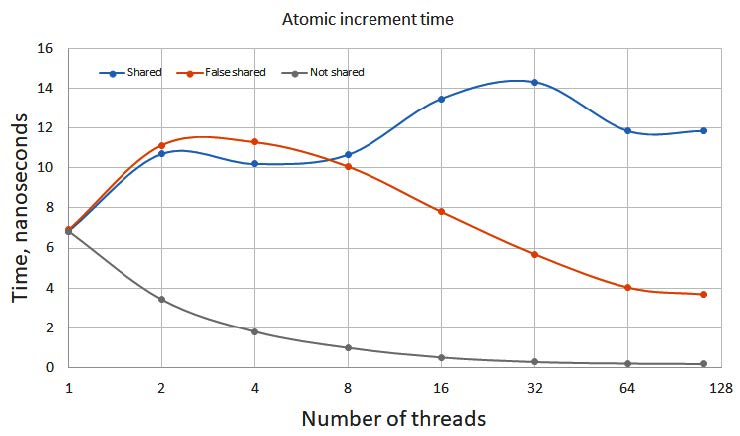
\includegraphics[width=0.9\textwidth]{content/1/chapter5/images/6.jpg}\\
图5.6 - 共享和非共享变量的原子增量时间
\end{center}

图5.4中的的\textbf{Shared}曲线为共享数据的基准测试曲线,另外两条曲线为不共享数据的基准测试曲线。线程上都有一个局部变量的基准测试标记为\textbf{Not shared},其行为如下:在两个线程上的计算时间比在一个线程上的计算时间少一半,在四个线程上的计算时间又减少了一半,以此类推。请记住,这是一个增量操作的平均时间:我们总共做了100万次增量,测量它所花费的总时间,然后除以100万。由于我们递增的变量不是在线程之间共享的,所以我们期望两个线程的运行速度是一个线程的两倍,所以\textbf{Not shared}的结果正是我们所期望的。另一个基准测试中,使用原子变量数组,但每个线程使用自己的数组元素,也没有共享数据。然而,其执行就像数据在线程之间共享一样,至少对于少量的线程是这样,所以我们称它为\textbf{伪共享}:没有什么是真正共享的,但程序的行为就像是共享的一样。

这个结果表明,数据共享成本高的原因比我们之前假设的要复杂:在伪共享的情况下,只有一个线程在操作每个数组元素,所以它不需要等待任何其他线程完成它的增量。然而,线程显然在彼此等待。为了理解这种异常现象,我们必须对缓存的工作方式进行更多的了解。

在多核或多处理器系统中,数据在处理器和内存之间移动的方式如图5.7所示。

\hspace*{\fill} \\ %插入空行
\begin{center}
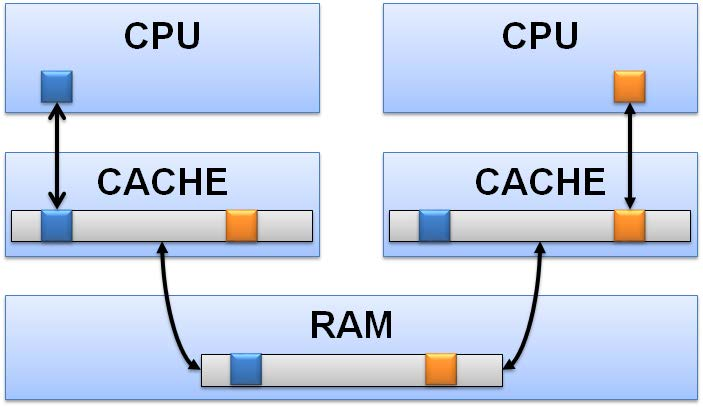
\includegraphics[width=0.9\textwidth]{content/1/chapter5/images/7.jpg}\\
图5.7 - 多核系统中CPU和内存之间的数据传输
\end{center}

处理器以字节或字的形式处理数据,这取决于变量的类型;在我们的例子中,一个\texttt{unsigned long}类型变量具有8字节。原子增量读取指定地址处的单个字,对其加1,然后写回。但是从哪里读呢?CPU只能直接访问L1缓存,因此只能从那里获取数据。数据如何从主存储器进入高速缓存?数据是通过内存总线复制的,而内存总线要宽得多。可以从内存复制到高速缓存并返回的最小数据量称为\textbf{缓存线}。在所有x86 CPU上,一条缓存线的大小为64字节。当CPU需要为一个原子事务锁定内存位置时,比如一个原子增量,CPU可能在写一个数据,并锁定整个缓存线:如果两个CPU可以在同一时间将同一缓存线写入内存,那么其中一个必然会覆盖另一个。注意,为了简单起见,我们在图5.7中只显示了一个级别的缓存层次结构,但这没有区别:数据以缓存线长度的形式通过所有级别的缓存。

现在可以解释我们观察到的伪共享:即使相邻的数组元素在线程之间并没有真正共享,但确实占用了相同的缓存线。当CPU请求独占访问一个数组元素时,它会锁定整个缓存线,阻止其他CPU访问其中的任何数据。顺便说一句,这解释了为什么图5.7中的伪共享在8个线程时看起来和真正的数据共享是一样的,但是在更多的线程时变得更快:写入的是8个字节的数据,所以它们中的8个可以放进同一个缓存线中。如果只有8个线程(或更少),那么在任何给定的时间,只有一个线程可以增加它的值,这与真正的共享一样。但是如果超过8个线程,数组至少占用两条缓存线,并且可以被两个独立的CPU锁住。所以,若有16个线程,那么就有两个线程可以向前移动,数组的一半对应一个线程。

另一方面,真正的非共享基准测试在每个线程的堆栈上分配原子变量。它们是完全独立的内存分配,由许多缓存线隔开。由于没有内存交互,这些线程可以完全独立地运行。

我们的分析表明,访问共享数据的高成本的真正原因是,必须维护对缓存线的独占访问,并确保所有CPU的缓存中有一致的数据:当一个CPU获得了独占访问权,并且更新了缓存线上的1位后,所有其他CPU的缓存线的复制就过期了。在其他CPU访问同一缓存线的数据之前,它们必须从主存中获取更新后的内容,这将花费相对较长的时间。

As we have seen, it doesn't really matter whether two threads try to access the same memory location or not, as long as they are competing for access to the same cache line. That exclusive cache line access is the origin of the high cost of shared variables. 

One may wonder whether the reason locks are expensive is also found in the shared data they contain (all locks must have some amount of shared data, that's the only way one thread can let another thread know that the lock is taken). A mutex lock is much more expensive than single atomic access, even on one thread, as we have seen in Figures 5.4 and 5.5. We can assume, correctly, that locking a mutex involves more work than just modifying one atomic variable. But why does this work take more time when we have more than one thread? Is it because the data is shared and needs exclusive access to the cache line? We leave it as an exercise to the reader to confirm that this is indeed so. The key to this experiment is to set up false sharing of locks: an array of locks such that each thread operates on its own lock, but they compete for the same cache line (of course, such per-thread locks don't actually protect anything from concurrent access, but all we want is the time it takes to lock and unlock them). The experiment is slightly more complex than you might think: the standard C++ mutex, std::mutex, is usually quite large, between 40 and 80 bytes depending on the OS. This means you can't fit even two of them into the same cache line. You have to do this experiment with a smaller lock, such as a spinlock or a futex.

We now understand why the cost of accessing the shared data concurrently is so high. This understanding gives us two important lessons. The first one is to avoid false data sharing when we attempt to create non-shared data. How can the unintended false sharing creep into our program? Consider the simple example we have studied throughout this chapter: accumulating a sum concurrently. Some of our approaches were slower than others, but they were all very slow (slower than the single-threaded program, or, at best, no faster). We understand that accessing shared data is expensive. So, what is less expensive? Not accessing the shared data, of course! Or at least not accessing it as often. There is no reason for us to access the shared sum value every time we want to add something to it: we can make all the additions locally, on the thread, and add them to the shared accumulator value once, at the very end. The code would look something like this: 

\hspace*{\fill} \\ %插入空行
\noindent
\textbf{04\_local\_incr.C}
\begin{lstlisting}[style=styleCXX]
// Global (shared) results
std::atomic<unsigned long> sum;
unsigned long local_sum[…];
// Per-thread work is done here
unsigned long& x = local_sum[thread_index];
for (size_t i = 0; i < N; ++i) ++x;
sum += x;
\end{lstlisting}

We have the global result, sum, that is shared between all threads and must be atomic (or protected by a lock). But each thread accesses this variable exactly once after all the work is done. Each thread uses another variable to hold the partial sum, only the values added on this thread (increments of 1 in our trivial case, but the performance is the same regardless of the values being added). We can create a large array to store these per-thread partial sums and give each thread a unique array element to work on. Of course, in this trivial example, we could just use a local variable, but in a real program, the partial results often need to be kept after the worker threads are done, and the final processing of these results is done elsewhere, perhaps by another thread. To simulate this kind of implementation, we use an array of per-thread variables. Note that these variables are just plain integers, not atomic: there is no concurrent access to them. Unfortunately, in the process, we fell into the trap of false sharing: the adjacent elements of the array are (usually) on the same cache line and, thus, cannot be accessed concurrently. This is reflected in the performance of our program:

%\hspace*{\fill} \\ %插入空行
\begin{center}
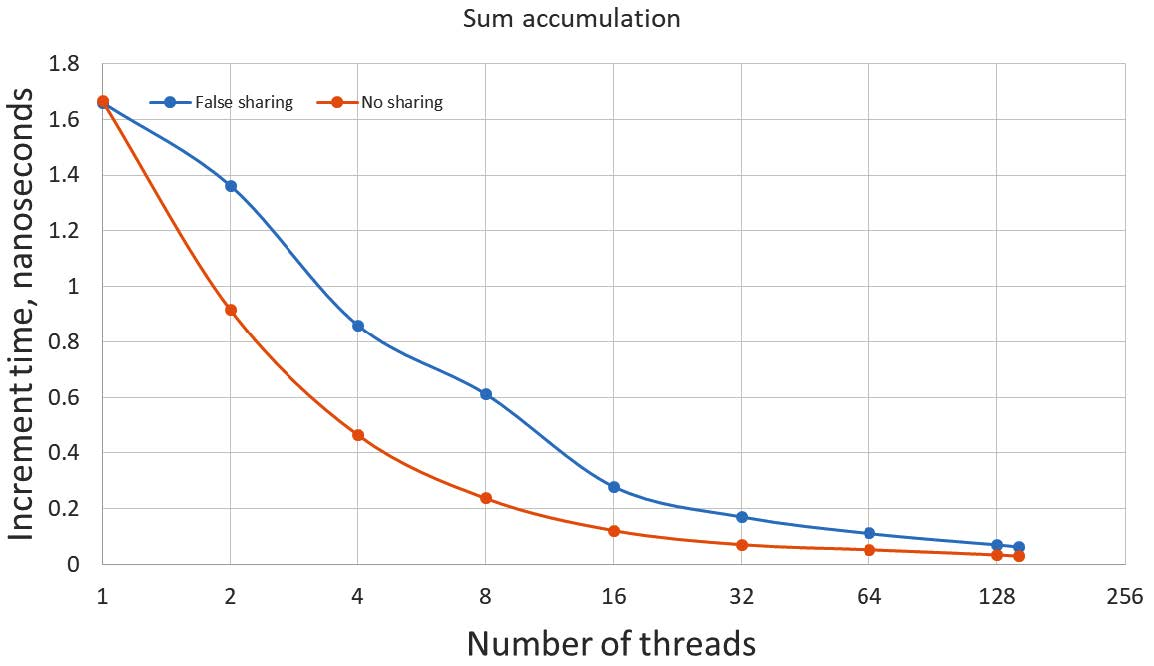
\includegraphics[width=0.9\textwidth]{content/1/chapter5/images/8.jpg}\\
Figure 5.8 – Sum accumulation with and without false sharing
\end{center}

As you can see in Figure 5.8, our program scales very poorly until we get to a very large number of threads. On the other hand, it scales perfectly, as expected, if we eliminate the false sharing by making sure the per-thread partial sums are at least 64 bytes apart (or simply using local variables in our case). While both programs become faster when we use more threads, the implementation that is not burdened by the false sharing remains approximately twice as fast.

The second lesson will become more important in the later chapters: since accessing shared variables concurrently is, comparatively, very expensive, an algorithm or an implementation that uses fewer shared variables will, in general, perform faster.

This statement may be confusing at the moment: by nature of the problem, we have some amount of the data that must be shared. We can do optimizations like the one we just did and eliminate unnecessary accesses to this data. But once this is done, the rest is the data we need to access to produce the desired results. How can there be more, or fewer, shared variables, then? To understand this, we have to realize that there is more to writing concurrent programs than protecting access to all shared data.






































